\section{Introduction}

This \cgal\ component implements a surface reconstruction method which takes as input point sets with oriented normals and computes an implicit function. We assume that the input points contain no outliers and little noise. The output surface mesh is generated by extracting an isosurface of this function with the \cgal\ Surface Mesh Generator~\cite{cgal:ry-gsddrm-06} or potentially with any other surface contouring algorithm.

% Insert image introduction.jpg/eps
\begin{center}
    % Image
    \begin{ccTexOnly}
        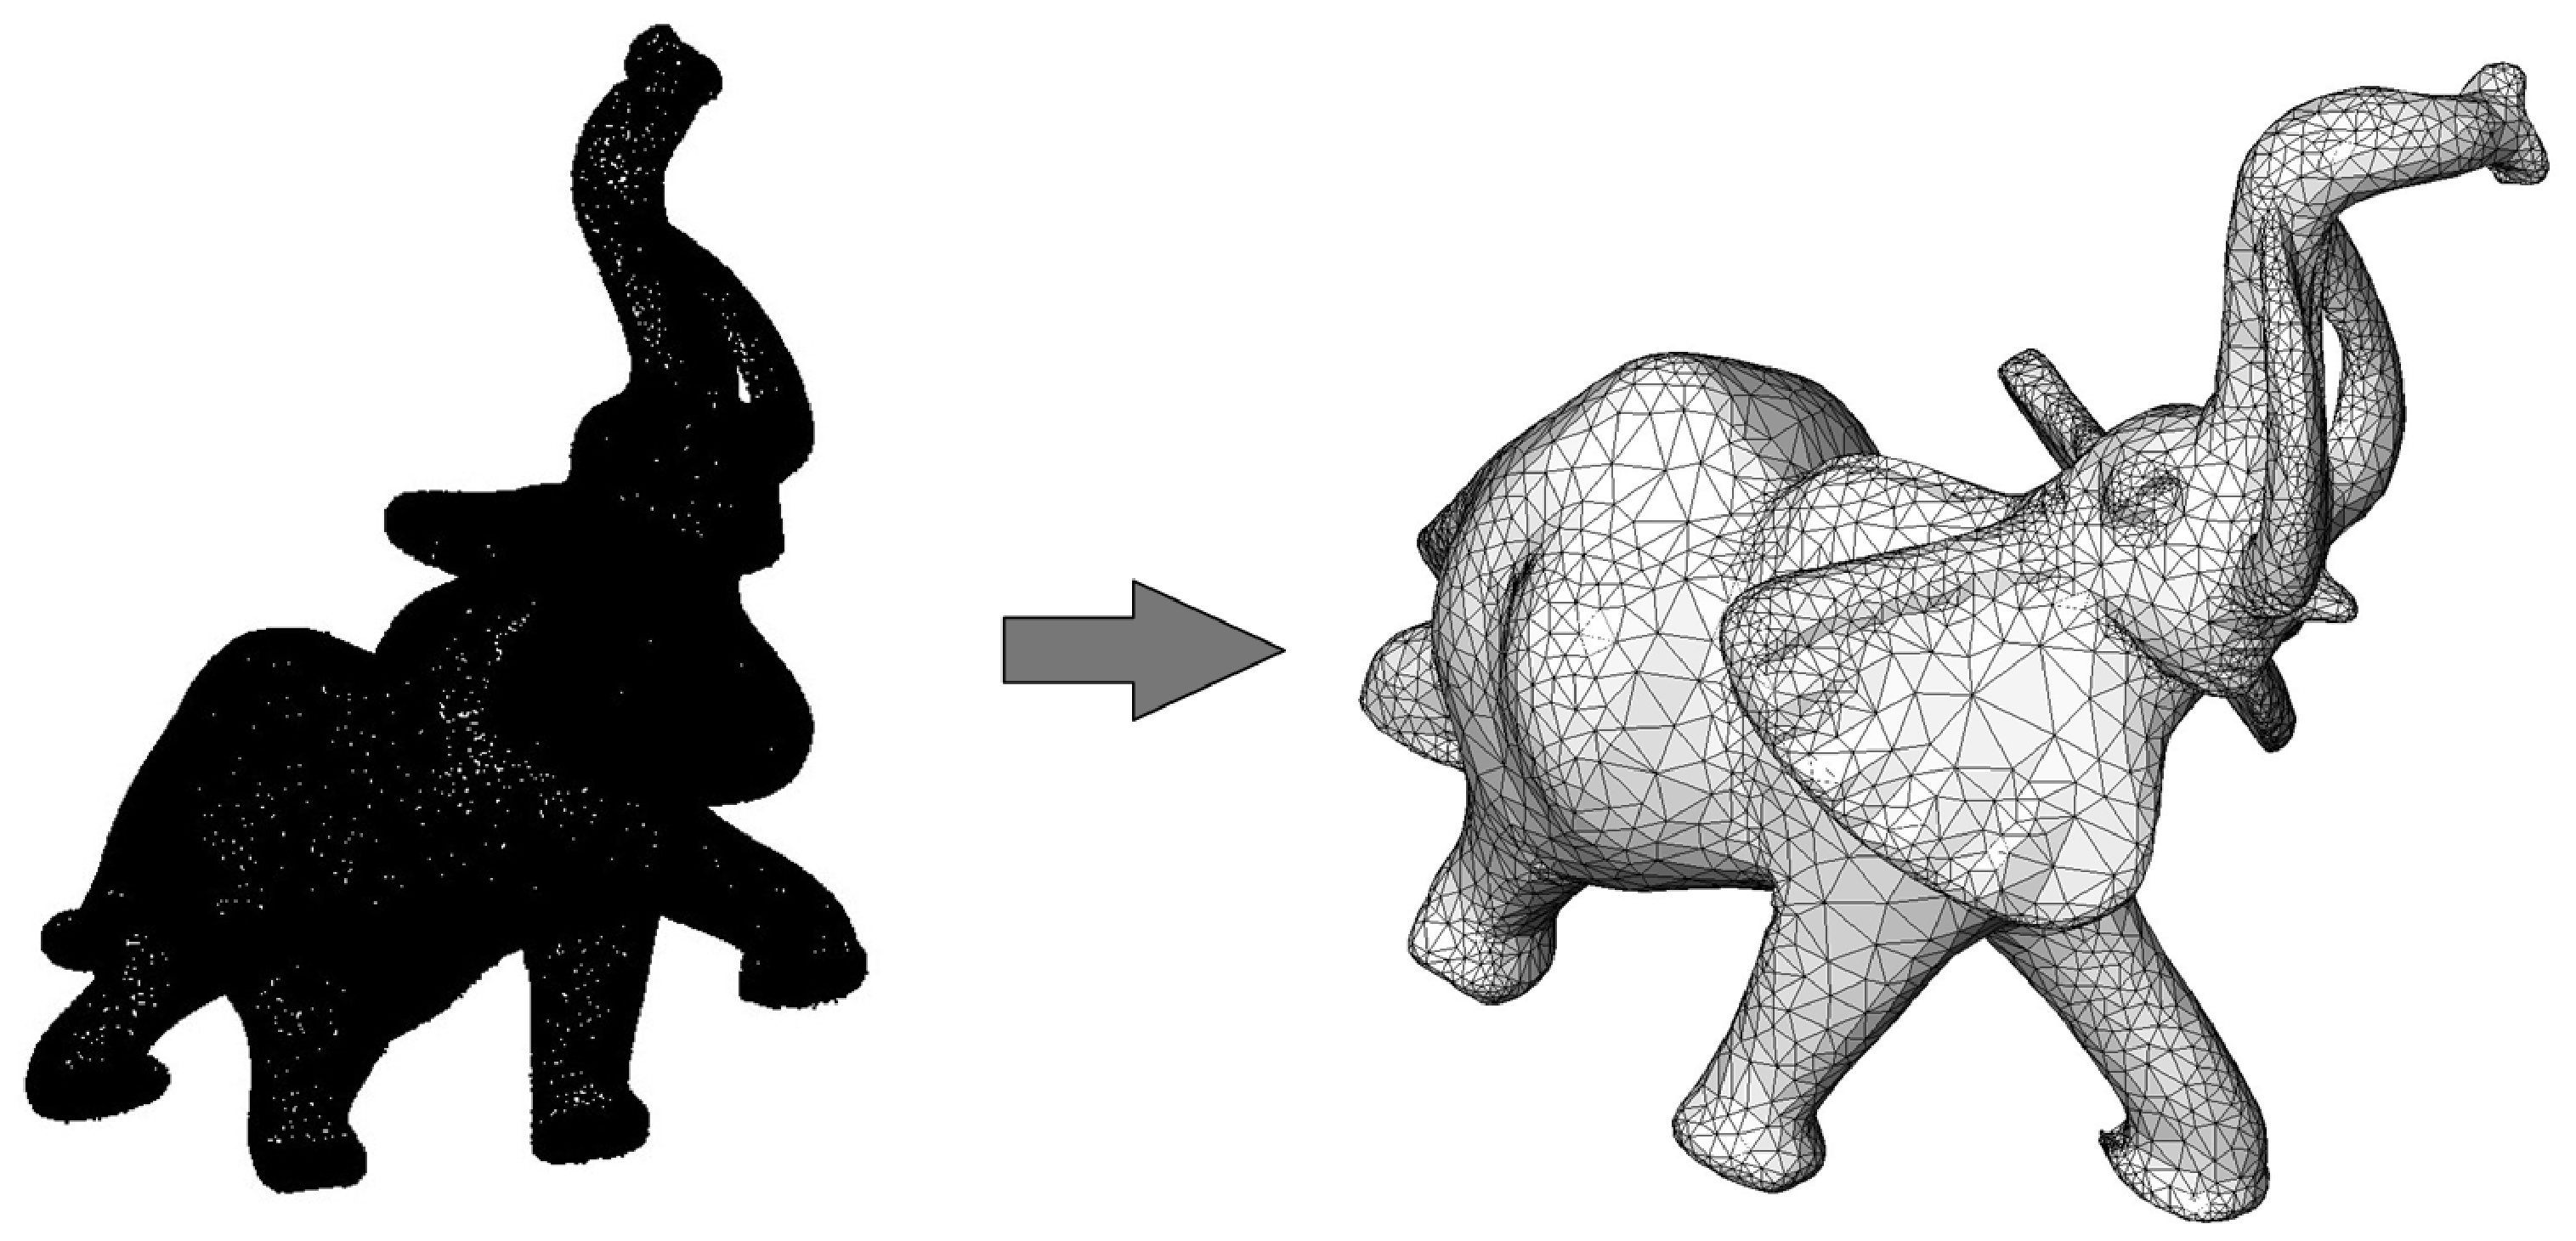
\includegraphics[width=1.0\textwidth]{Surface_reconstruction_points_3/introduction} % omit .eps suffix
    \end{ccTexOnly}
    \begin{ccHtmlOnly}
        <img style="max-width: 70%;" border=0 src="./introduction.jpg"><P>
    \end{ccHtmlOnly}
    % Title
    \begin{figure}[h]
        \caption{Poisson surface reconstruction.
                 Left: 17K points sampled on the statue of an
                 elephant with a Minolta laser scanner.
                 Right: reconstructed surface mesh.}
        \label{Surface_reconstruction_points_3-fig-introduction}
    \end{figure}
\end{center}

More specifically, the core surface reconstruction algorithm consists of computing an implicit function which is an approximate indicator function of the inferred solid (Poisson Surface Reconstruction - referred to as Poisson). Poisson is a two steps process: it requires solving for the implicit function before function evaluation.


\section{Common Reconstruction Pipeline}

Surface reconstruction from point sets is often a sequential process with the following steps: 1) Scanning and scan alignment produce a set of points or points with normals; 2) Outlier removal; 3) Simplification to reduce the number of input points; 4) Smoothing to reduce noise in the input data; 5) Normal estimation and orientation when the normals are not already provided by the acquisition device; and 6) Surface reconstruction. \\
\cgal\ provides algorithms for all steps listed above except alignment. \\
Chapter \ccc{Point_set_processing_3} \ref{chap:point_set_processing_3} describes algorithms to pre-process the point set before reconstruction with functions devoted to the simplification, outlier removal, smoothing, normal estimation and normal orientation.

% Insert image pipeline.jpg/eps
\begin{center}
    % Image
    \begin{ccTexOnly}
        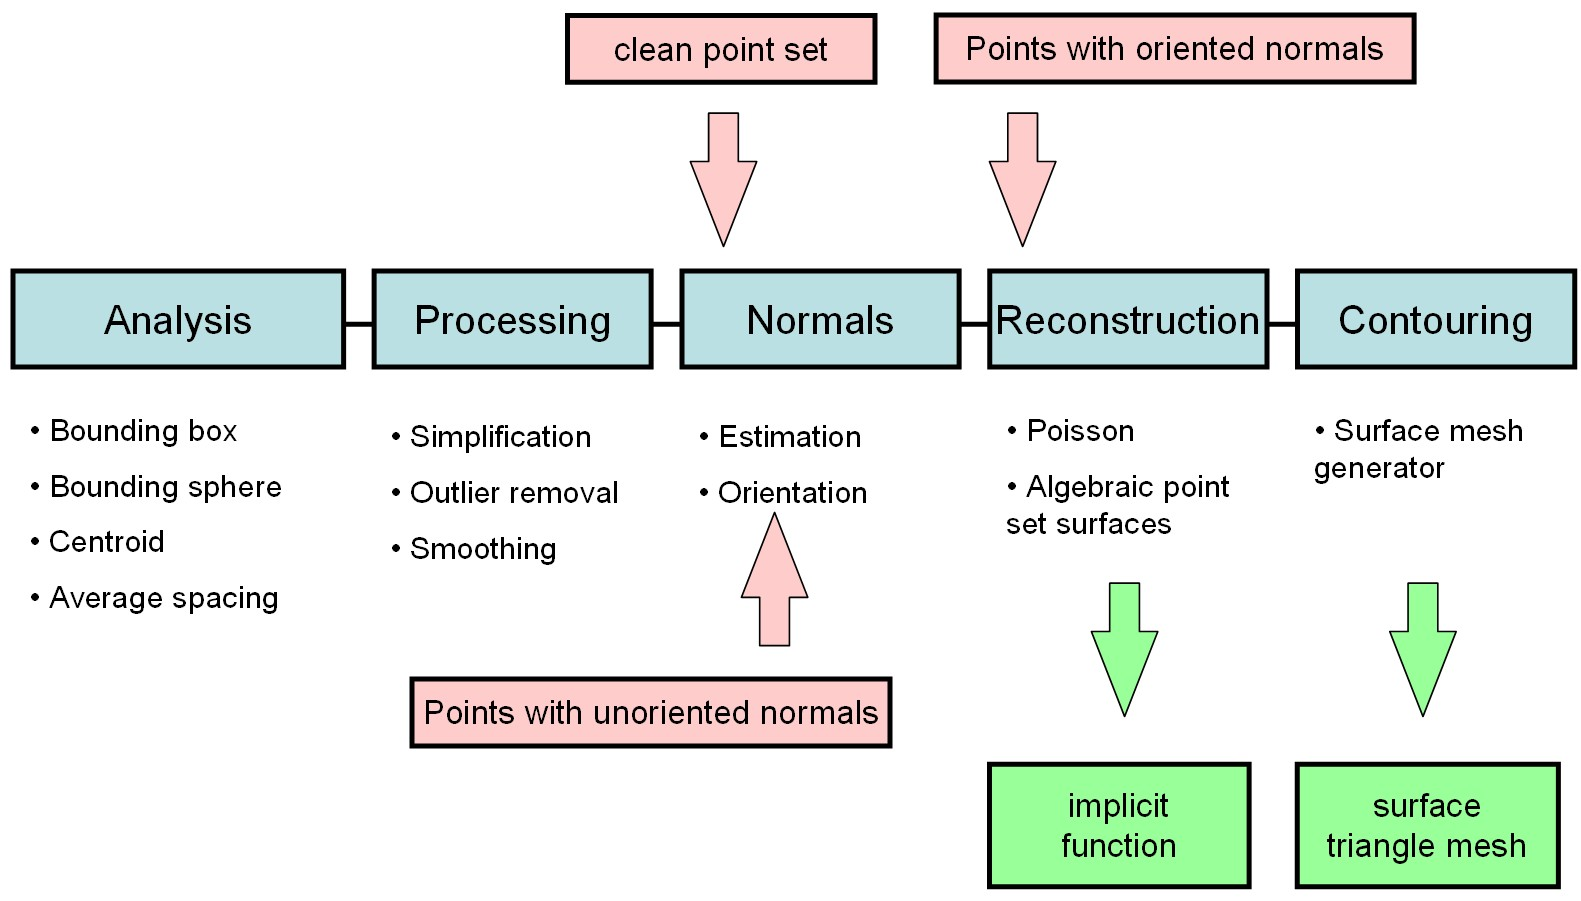
\includegraphics[width=1.0\textwidth]{Surface_reconstruction_points_3/pipeline} % omit .eps suffix
    \end{ccTexOnly}
    \begin{ccHtmlOnly}
        <img style="max-width: 100%;" border=0 src="./pipeline.jpg"><P>
    \end{ccHtmlOnly}
    % Title
    \begin{figure}[h]
        \caption{Common surface reconstruction pipeline.}
        \label{Surface_reconstruction_points_3-fig-pipeline}
    \end{figure}
\end{center}

